\section{Results and Discussion}
\label{sec:results}

This section presents the consolidated quantitative and computational analyses across the evaluated LLFF scenes. Table \ref{tab:super_results} summarizes the global averages for visual fidelity, temporal efficiency, and memory footprint. The results reveal critical trade-offs between generalization, optimization stability, and hardware constraints.

\subsection{Visual Fidelity and Architectural Inertia}
The per-scene architectures demonstrated vastly superior visual reconstruction capabilities. Nerfacto established the performance upper bound, achieving a global average of 27.11 dB PSNR and 0.875 SSIM. In contrast, the generalizable models struggled significantly with the sparse constraints of the LLFF dataset. 

A notable phenomenon observed in the consolidated data is the performance degradation during Test-Time Adaptation (TTA). Counterintuitively, fine-tuning the generalizable models on sparse views slightly decreased their PSNR compared to their Zero-Shot baselines. PixelNeRF dropped from 6.62 dB to 6.38 dB, while GNT decreased from 10.73 dB to 10.42 dB. This behavior suggests a representational collapse or "architectural inertia", where the lack of dense geometric priors and depth regularization during few-shot fine-tuning causes the networks to overfit the sparse inputs, actively destroying the generalized prior they possessed in the Zero-Shot regime.

\subsection{Computational Trade-offs}
From a systemic viability perspective, a severe dichotomy emerges between inference latency and training overhead. While generalizable models bypass extensive optimization (requiring only seconds for Zero-Shot inference or $\sim$7 minutes for TTA), their volumetric feature aggregation mechanisms result in catastrophic inference bottlenecks, yielding rendering speeds below 0.02 FPS. 

Conversely, the explicit multiscale hash representations of the per-scene models proved vastly more efficient during runtime. Despite requiring lengthier convergence periods (from $\sim$9 minutes for Nerfacto up to $\sim$32 minutes for Instant-NGP), they achieve inference rates up to $97\times$ faster than generalizable approaches (0.388 FPS). Furthermore, the hash-based models exhibit a highly optimized dynamic memory footprint, with Instant-NGP operating at just 1.09 GB of VRAM during inference, solidifying per-scene methods as the most viable path for hardware-constrained deployments despite the initial training cost.


\begin{figure}[!t]
\centering
% Lembre-se de ajustar o caminho da imagem se necessário
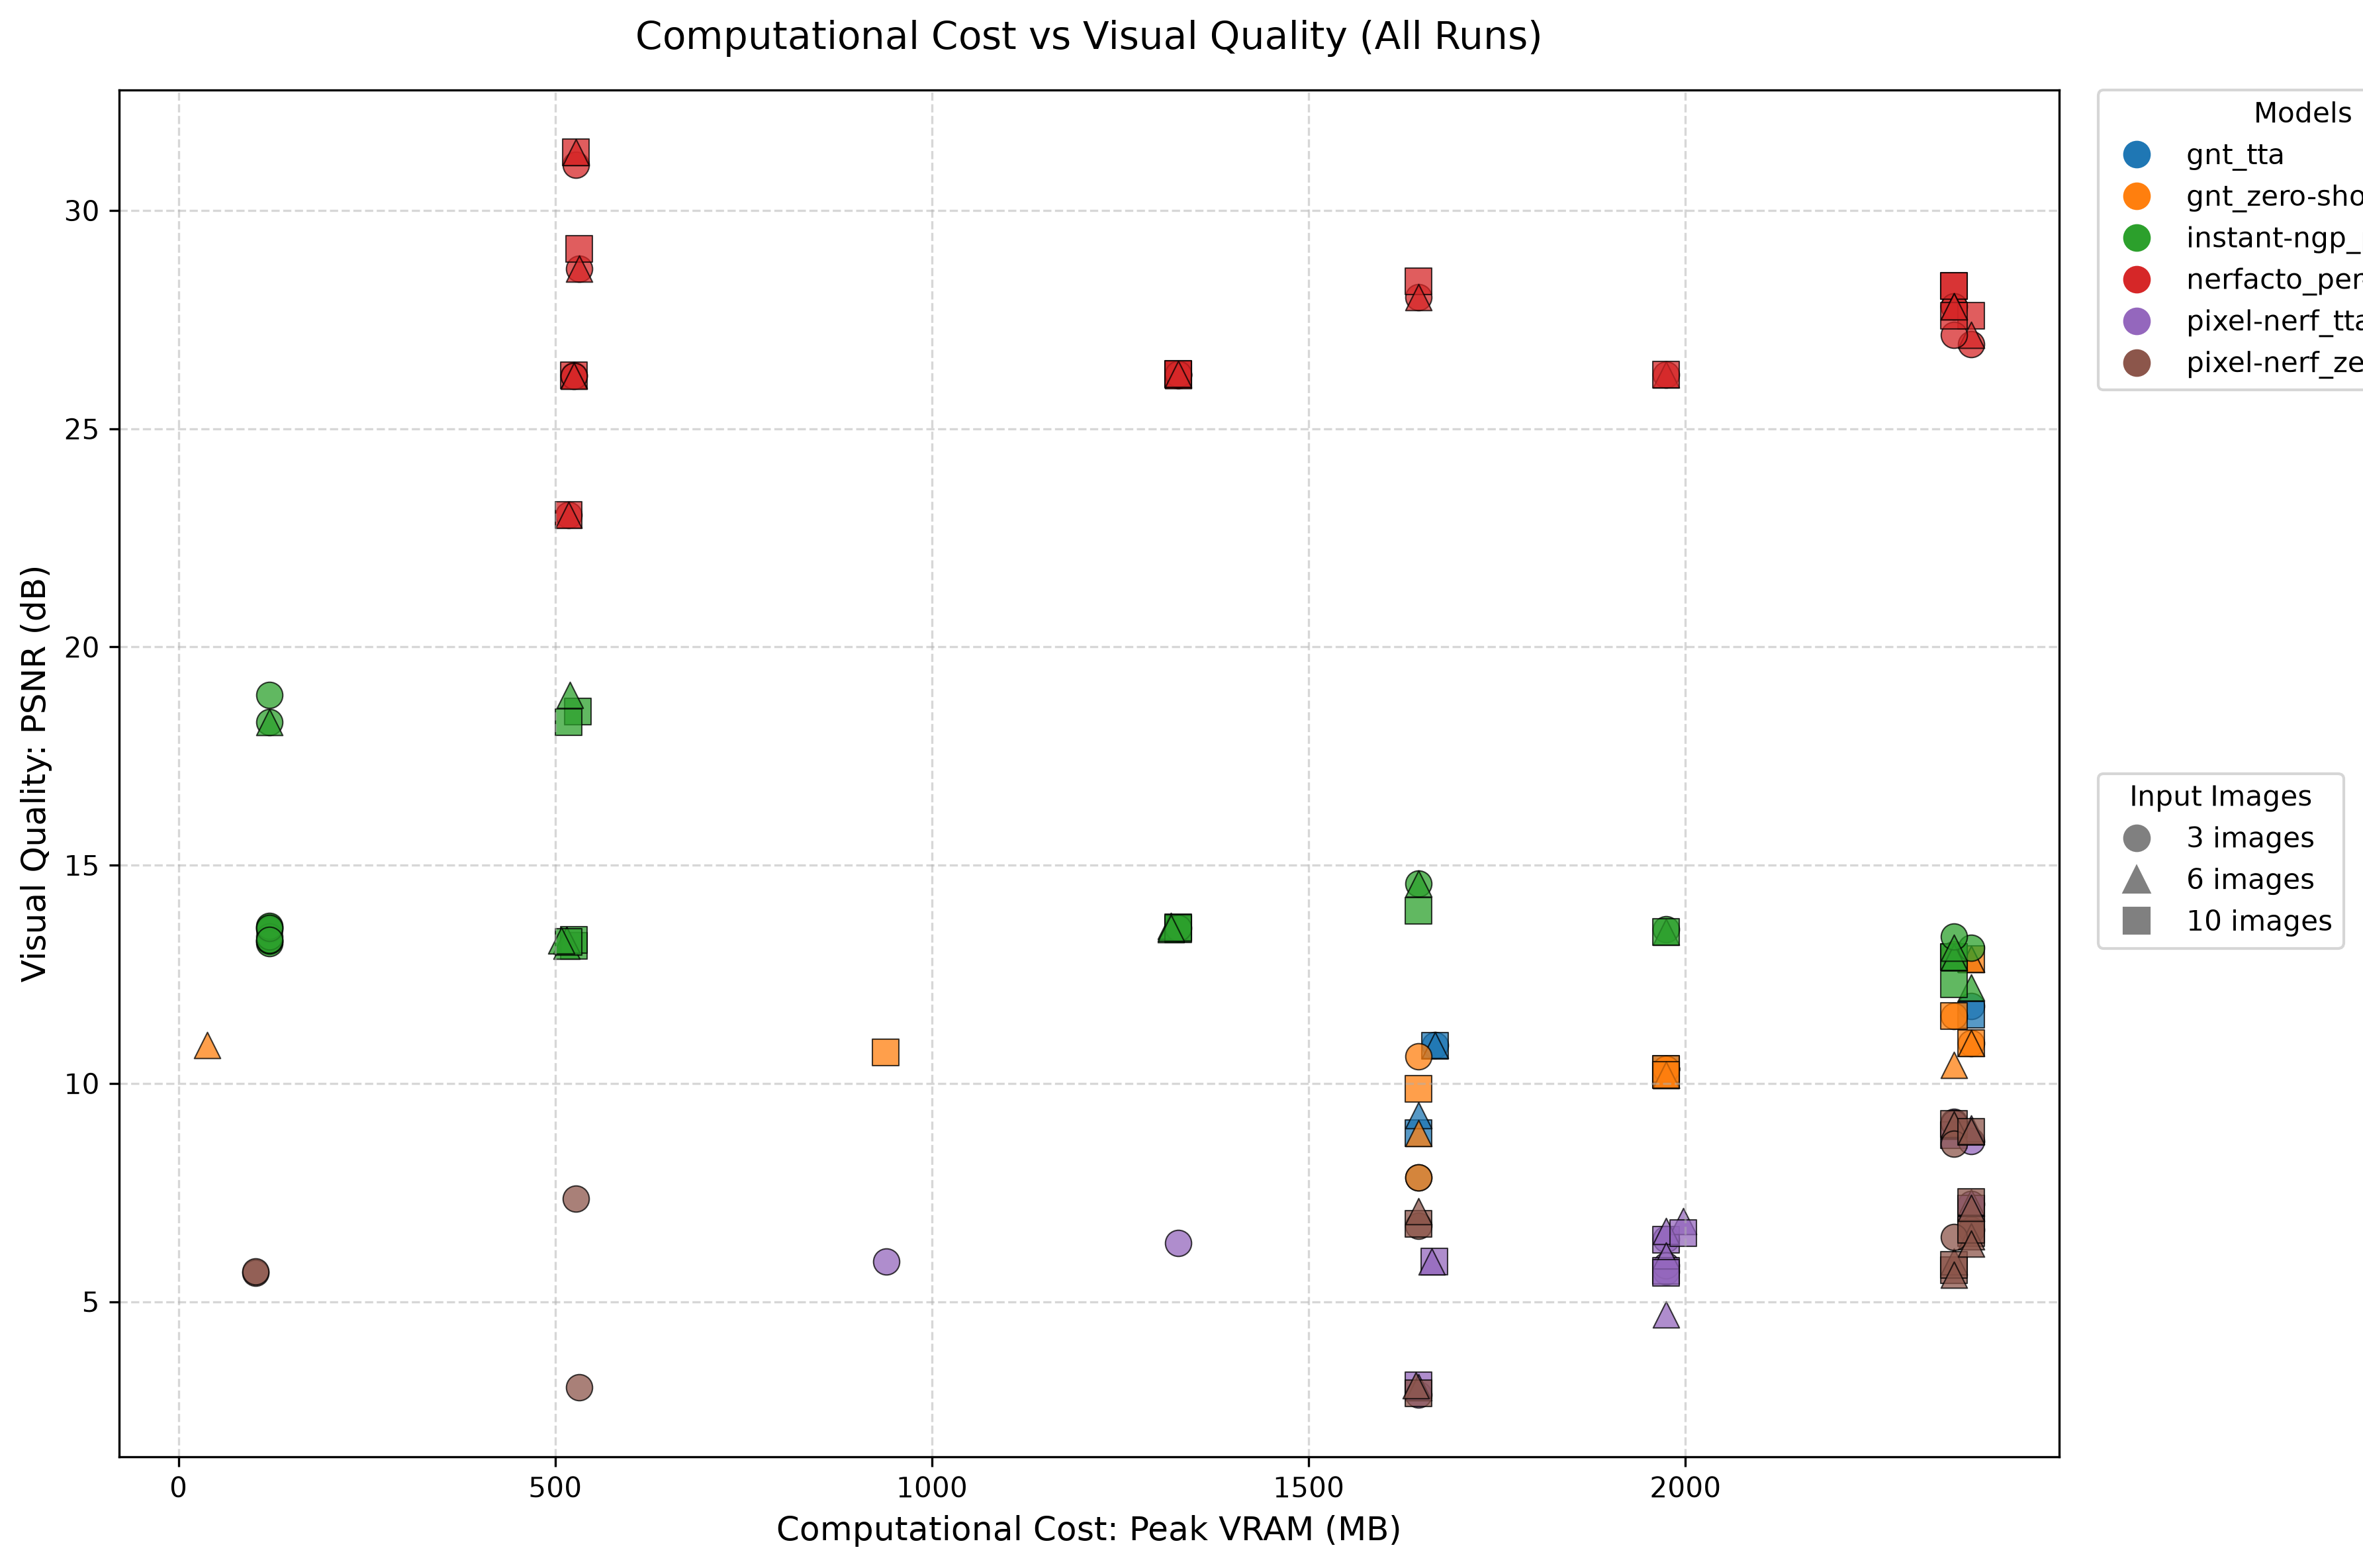
\includegraphics[width=\linewidth]{img/vram_vs_psnr_all_runs_plot.png}
\caption{Trade-off between visual fidelity (PSNR) and computational cost (Peak VRAM) across all evaluated scenes and regimes. The top-left quadrant represents the ideal operational region (high quality, low memory footprint), which is heavily dominated by per-scene hash-based architectures.}
\label{fig:vram_vs_psnr}
\end{figure}
\begin{table*}[!t]
\centering
\caption{Consolidated quantitative results across the LLFF dataset. Metrics represent the global average. Training time reflects the fine-tuning phase for TTA and full convergence for Per-Scene models. VRAM Peak denotes dynamic memory allocation during inference.}
\label{tab:super_results}
\resizebox{\textwidth}{!}{%
\begin{tabular}{llcccccc}
\toprule
\textbf{Paradigm} & \textbf{Model \& Regime} 
  & \textbf{PSNR (dB) $\uparrow$} 
  & \textbf{SSIM $\uparrow$} 
  & \textbf{LPIPS $\downarrow$} 
  & \textbf{Train / TTA Time} 
  & \textbf{Inference (FPS) $\uparrow$} 
  & \textbf{VRAM Peak (GB) $\downarrow$} \\
\midrule
\multirow{4}{*}{\textbf{Generalizable}} 
 & PixelNeRF (Zero-Shot) & 6.62  & 0.093 & 0.814 & $\sim$22 s   & 0.004 & 1.93 \\
 & PixelNeRF (TTA)       & 6.38  & 0.071 & 0.801 & 4 min 23 s   & 0.006 & 1.97 \\
 \cmidrule{2-8}
 & GNT (Zero-Shot)       & 10.73 & 0.300 & 0.760 & $\sim$9 s    & 0.014 & 1.94 \\
 & GNT (TTA)             & 10.42 & 0.336 & 0.724 & 7 min 19 s   & 0.015 & 1.93 \\
\midrule
\multirow{2}{*}{\textbf{Per-Scene}}     
 & Instant-NGP (100\%)   & 14.06 & 0.442 & 0.498 & 31 min 51 s  & 0.199 & \textbf{1.09} \\
 & Nerfacto (100\%)      & \textbf{27.11} & \textbf{0.875} & \textbf{0.171} & 8 min 57 s   & \textbf{0.388} & 1.43 \\
\bottomrule
\end{tabular}%
}
\end{table*}

\subsection{Qualitative Analysis}

The qualitative assessment visually corroborates the quantitative metrics, specifically illustrating the boundaries of each architectural paradigm. For visual clarity, we synthesized novel views matching the exact poses from the test set using perspective projection.

Figure \ref{fig:comparacao_qualitativa} highlights the severe disparities in reconstruction quality on the highly detailed \textit{fern} scene. As visually evident, neither PixelNeRF nor GNT achieved proper convergence. PixelNeRF produced renderings with intense isotropic blurring, a typical artifact indicating the network's failure to accurately localize 2D projected features across extremely sparse views. GNT, on the other hand, demonstrated a complete generalization failure regarding the \textit{in-the-wild} characteristics of the scene. This resulted in a representational visual collapse—heavily distorting the volumetric geometry into noise—which persisted even after the 10-view Test-Time Adaptation (TTA).

Conversely, the per-scene architectures successfully captured the intricate foliage geometry. While Instant-NGP exhibited minor volumetric density fluctuations (floaters) in sparsely covered peripheral regions, Nerfacto produced a highly faithful reconstruction, preserving high-frequency details directly matching the native resolution of the Ground Truth.

\begin{figure}[!t]
    \centering
    % Row 1: Ground Truth (Centered)
    \begin{subfigure}[b]{0.48\linewidth}
        \centering
        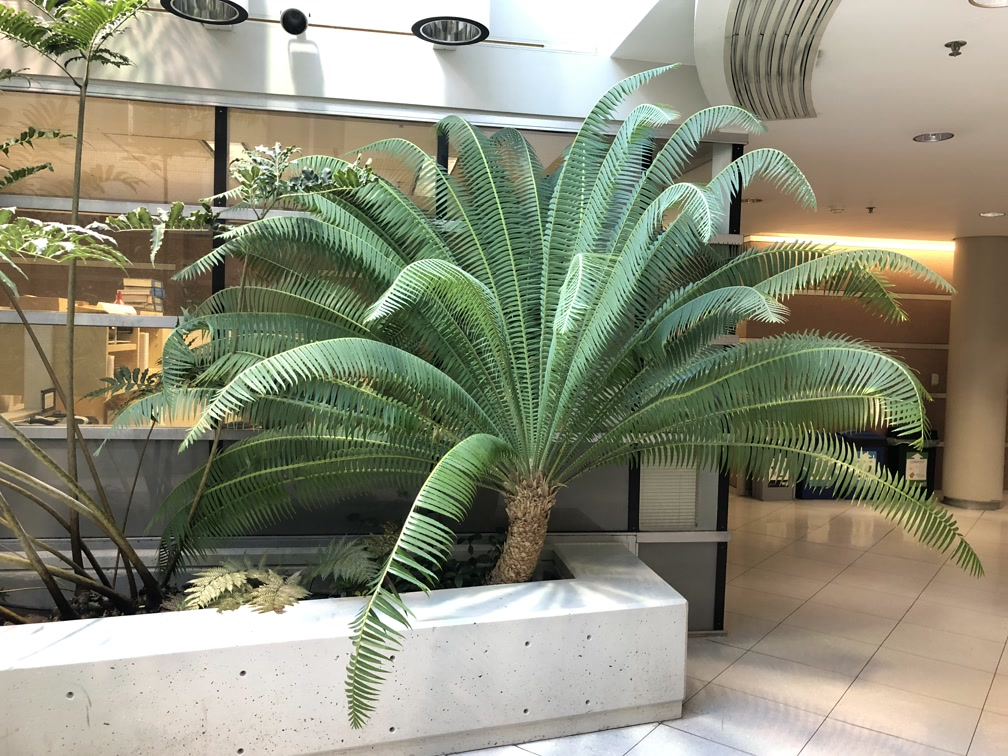
\includegraphics[width=\linewidth]{img/gt.jpg}
        \caption*{Ground Truth}
    \end{subfigure}
    
    \vspace{2mm} % Vertical spacing between rows

    % Row 2: Generalizable Models (The ones that failed)
    \begin{subfigure}[b]{0.48\linewidth}
        \centering
        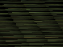
\includegraphics[width=\linewidth]{img/pixel-nerf.png}
        \caption*{PixelNeRF (TTA 10)}
    \end{subfigure}\hfill
    \begin{subfigure}[b]{0.48\linewidth}
        \centering
        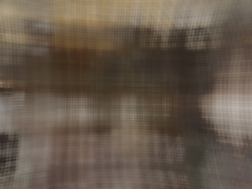
\includegraphics[width=\linewidth]{img/gnt.png}
        \caption*{GNT (TTA 10)}
    \end{subfigure}
    
    \vspace{2mm}
    
    % Row 3: Per-Scene Models (The successful ones)
    \begin{subfigure}[b]{0.48\linewidth}
        \centering
        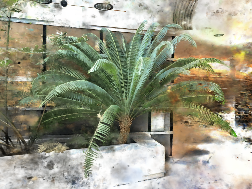
\includegraphics[width=\linewidth]{img/instant-ngp.png}
        \caption*{Instant-NGP (Per-Scene)}
    \end{subfigure}\hfill
    \begin{subfigure}[b]{0.48\linewidth}
        \centering
        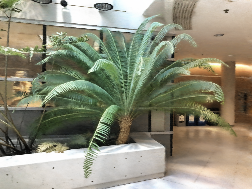
\includegraphics[width=\linewidth]{img/nerfacto.png}
        \caption*{Nerfacto (Per-Scene)}
    \end{subfigure}

    \caption{Qualitative comparison on the \textit{fern} scene. Generalizable architectures (PixelNeRF and GNT) failed to converge under sparse constraints, resulting in severe blurring and visual collapse. In contrast, per-scene optimization models (Instant-NGP and Nerfacto) successfully reconstructed the complex geometry.}
    \label{fig:comparacao_qualitativa}
\end{figure}
